% PLANTILLA APA7
% Creado por: Isaac Palma Medina
% Última actualización: 25/07/2021
% @COPYLEFT

% Fuentes consultadas (todos los derechos reservados):
% Normas APA. (2019). Guía Normas APA. https://normas-apa.org/wp-content/uploads/Guia-Normas-APA-7ma-edicion.pdf
% Tecnológico de Costa Rica [Richmond]. (2020, 16 abril). LaTeX desde cero con Overleaf (1 de 3) [Vídeo]. YouTube. https://www.youtube.com/watch?v=kM1KvHVuaTY Weiss, D. (2021).
% Formatting documents in APA style (7th Edition) with the apa7 LATEX class. https://ctan.math.washington.edu/tex-archive/macros/latex/contrib/apa7/apa7.pdf @COPYLEFT

%+-+-+-+-++-+-+-+-+-+-+-+-+-++-+-+-+-+-+-+-+-+-+-+-+-+-+-+-+-+-++-+-+-+-+-+-+-+-+-+

% Preámbulo
\documentclass[stu, 12pt, letterpaper, donotrepeattitle, floatsintext, natbib]{apa7}
\usepackage[utf8]{inputenc}
\usepackage[T1]{fontenc}
\usepackage{comment}
\usepackage{marvosym}
\usepackage{graphicx}
\usepackage{float}
\usepackage[normalem]{ulem}
\usepackage[english]{babel}
\usepackage{booktabs}
\usepackage{tabularx}
\usepackage{array}
\usepackage{amsmath}
\usepackage{listings}
\usepackage{xcolor}
\usepackage{tikz}
\usetikzlibrary{shapes.geometric, arrows.meta, positioning, fit, backgrounds}

\useunder{\uline}{\ul}{}
\hypersetup{hidelinks}
\newcommand{\myparagraph}[1]{\paragraph{#1}\mbox{}\\}
\sloppy
\newcommand{\EventsTotal}{8,000}
\newcommand{\EventsPerYear}{470.6}
\newcommand{\FlashShare}{80.4}
\newcommand{\DamageBn}{49.0}
\newcommand{\Deaths}{432}
\newcommand{\GovRows}{399}
\newcommand{\StoryRows}{2,294}
\newcommand{\GovFile}{governance\_20261117\_192000.parquet}
\newcommand{\StoryFile}{storytelling\_20261117\_192000.parquet}

% Configuración para bloques de código
\lstset{
  basicstyle=\ttfamily\footnotesize,
  breaklines=true,
  frame=single,
  backgroundcolor=\color{gray!8},
  rulecolor=\color{gray!40},
  xleftmargin=6pt,
  xrightmargin=6pt,
  columns=fullflexible
}

% Airflow screenshots: put the PNG files in screenshots/ and recompile.
\newcommand{\shot}[2]{\begin{figure}[H]\centering\caption{#2}
  \IfFileExists{screenshots/#1}{\includegraphics[width=0.95\textwidth]{screenshots/#1}}%
  {\fbox{\parbox{0.9\textwidth}{\centering\vspace{1cm}\textcolor{red}{\textbf{Screenshot pending:} \texttt{screenshots/\detokenize{#1}}}\vspace{1cm}}}}
  \end{figure}}

% Portada
\thispagestyle{empty}
\title{\Large Silver-to-Gold Pipeline, Governance KPIs, and Storytelling Definition \\ \large Workshop No. 3: Flood Monitoring and Risk System (Texas, USA)}
\author{Oscar Durán (20212020080) \\ Laura Natalia Pardo (20221020146) \\ Nicolás Romero (20222020023)}
\affiliation{Universidad Distrital Francisco José de Caldas}
\course{Data Analysis Programming (2026-III)}
\professor{Carlos Andrés Sierra}
\duedate{Bogotá, D.C., November 2026}

\begin{document}
% long code identifiers may break after an underscore inside narrow table columns
\let\oldunderscore\_
\renewcommand{\_}{\oldunderscore\allowbreak}
\maketitle

% Índices
\pagenumbering{roman}
\renewcommand\contentsname{\large Contents}
\tableofcontents
\setcounter{tocdepth}{2}
\newpage

% Cuerpo
\pagenumbering{arabic}

\noindent \textbf{Team 2 Members:} Oscar Durán (20212020080), Laura Natalia Pardo (20221020146), Nicolás Romero (20222020023) \\
\textbf{Professor:} Eng. Carlos Andrés Sierra, M.Sc. \\
\textbf{Location \& Date:} Bogotá, D.C., November 2026 \\
\textbf{GitHub Repository:} \url{https://github.com/natcastill/flood-monitoring-team2}

% ===========================================================================
\section{\large 1. Executive Summary}
Workshop~2 left the Flood Monitoring and Risk System with a working Bronze ingestion DAG and a FileSensor-triggered Silver DAG. In this workshop we reviewed every Bronze JSON file and every Silver Parquet file those DAGs produced, improved both pipelines from what we observed, and built the Gold layer with PySpark \citep{zaharia2016, spark2026}.

\textbf{Pipeline improvements.} The review found ten data-quality problems that the Workshop~2 design did not anticipate (W3-1 to W3-10, Section~2). Three examples:
\begin{itemize}
    \item the hourly rainfall of the NWS stations was null in 100\,\% of the Silver rows, because the API leaves it empty in dry METAR hours; it is now read from the METAR text;
    \item 1.6\,\% of the Storm Events narratives contained broken characters (U+FFFD), and the episode narrative was repeated in 75\,\% of the rows, which inflated the keyword counts;
    \item every Bronze run downloaded the same 7-day window of alerts again (66\,\% of the alert rows were duplicates); the Bronze DAG now asks only for new alerts.
\end{itemize}
Silver was then rebuilt from the immutable Bronze files with preprocessing v0.3, so all Silver files share one schema per topic.

\textbf{Gold layer.} A new Airflow DAG, \texttt{gold\_flood\_processing\_dag}, runs PySpark in local mode inside the Docker stack. It reads the whole \texttt{datalake\_silver/} folder as one DataFrame per topic and writes two timestamped Parquet files to \texttt{datalake\_gold/}:
\begin{itemize}
    \item a \textbf{governance summary} (\GovRows{} rows) with 23 KPI types in seven quality dimensions: completeness, uniqueness, validity, text, accuracy, timeliness and volume \citep{wang1996, batini2009};
    \item a \textbf{storytelling summary} (\StoryRows{} rows) with 15 sections, each mapped to a Workshop~1 user story and to one element of the Workshop~4 dashboard.
\end{itemize}

\textbf{The story.} The functional user is the emergency analyst of Workshop~1. The dashboard answers: \emph{where and when does Texas flood, what do floods do, and is today unusual?} Since 2010 there were \EventsTotal{} flood records in Texas (\EventsPerYear{} per year); \FlashShare\,\% were flash floods, with USD~\DamageBn{}~billion of reported property damage and \Deaths{} deaths. The Gold run also computes the Flood Risk Index per county proposed in Workshop~1, and back-tests it against 16 years of history. The back-test showed that the original rule raises too many false alarms, which we document as a finding for Workshop~4.

% ===========================================================================
\section{\large 2. Pipeline Improvements Based on Experimentation}
We reviewed the nine Bronze files of 16--17 November 2026 and the Silver files of Workshop~2 with \texttt{notebooks/03\_data\_quality\_findings.ipynb}. Table~\ref{tab:improvements} lists what we observed, what we changed and why. Each change is labeled in the code (\texttt{W3-n}).

\begin{table}[H]
\centering
\scriptsize
\caption{Before/after comparison of the Bronze and Silver pipelines (Workshop~2 = before, Workshop~3 = after).}
\label{tab:improvements}
\begin{tabularx}{\textwidth}{>{\raggedright\arraybackslash}p{0.8cm} >{\raggedright\arraybackslash}p{3.4cm} >{\raggedright\arraybackslash}p{4.4cm} >{\raggedright\arraybackslash}X}
\toprule
\textbf{\#} & \textbf{Observed in Workshop~2} & \textbf{Change in Workshop~3} & \textbf{Why / effect} \\
\midrule
W3-1 Silver & \texttt{precip\_1h\_mm} was null in 100\,\% of the rows, METAR hours included. The raw JSON shows that 5-minute reports do not even contain the key, and METAR reports carry it with \texttt{value = null}. & The rainfall is read from the METAR \texttt{rawMessage}: the \texttt{Pxxxx} group gives hundredths of an inch; an automated (\texttt{AO2}) hourly report without it means 0~mm; \texttt{PNO} means the gauge is down \citep{ofcm2019}. New columns \texttt{precip\_source}, \texttt{precip\_inferred\_zero}. & Null rate in METAR hours: 100\,\% $\rightarrow$ 0\,\%. 5-minute reports stay \texttt{NULL} (still not 0~mm). US2 and the index can now use the hourly rainfall. \\
\addlinespace
W3-2 Silver & 6--13\,\% of the METAR reports of KAUS, KSAT and KCRP end with \texttt{\$}. & New flag \texttt{maintenance\_flag}. & The \texttt{\$} sign means the station needs maintenance: its values deserve less trust. \\
\addlinespace
W3-3 Silver & 125 Storm Events records (1.6\,\%) contain the replacement character U+FFFD (e.g., ``M\textbf{??}xico'', ``1\textbf{???}2 inches'', ``city\textbf{???}s''). & \texttt{repair\_encoding()}: known words repaired, digit ranges become ``1-2'', possessives become ``'s'', other U+FFFD removed; accents folded to ASCII; flag \texttt{encoding\_repaired}. & In Workshop~2 the punctuation step turned them into junk tokens such as ``xico''. \\
\addlinespace
W3-4 Silver & Top keywords were generic: ``texas'', ``county'', ``produced'', ``upper'', ``level'', ``reported'', ``moved'' (Table~\ref{tab:kw}); road identifiers (``FM 1960'', ``US 59'') left tokens such as ``us'' or ``fm''; boilerplate sentences such as ``The cost of damage is a very rough estimate'' appeared in 214 events. & Domain stop-word list (117 words), road identifiers become ``road'', clock times and ordinal dates removed, boilerplate sentences removed, tokens with digits or fewer than 3 letters dropped, narratives split into sentences. & Keywords now describe impacts (``water rescues'', ``low water'', ``road closures'') instead of how the record was written. \\
\addlinespace
W3-5 Silver & The episode narrative was concatenated to the event narrative, but it is copied into every event of the same episode (75.3\,\% of the rows repeat another row's episode text). & Keywords and word counts come from the event narrative; the episode narrative is kept in its own column and used only when the event narrative is empty (61 events, \texttt{narrative\_source}). & Mean narrative length 126 $\rightarrow$ 31 words; no keyword is counted several times for one storm. \\
\addlinespace
W3-6 Silver & New outlier pattern: 115 events last more than 72~h (up to 720~h = 30 days). & \texttt{duration\_hours} and \texttt{is\_outlier\_duration} (IQR, $k=3$, on $\log(1+h)$); negative durations set to \texttt{NULL}. & Long river floods are real: they are flagged and kept, so averages can exclude them. \\
\addlinespace
W3-7 Silver & Alert descriptions start with ``\texttt{* WHAT...}'', ``\texttt{* WHERE...}'', ``\texttt{* IMPACTS...}''; the \texttt{reference\_ids} were URLs (``\texttt{https://api.weather.gov/\allowbreak alerts/\allowbreak urn:...}'') while \texttt{alert\_id} is the bare URN, so an Update or Cancel never matched its alert. & Section markers removed; \texttt{reference\_ids} use the \texttt{identifier} field (29 of 33 references now match an alert in Silver); new \texttt{counties} list and \texttt{ugc\_type}; raw \texttt{headline} kept for display. & Gold can drop superseded messages and show only the alerts in effect (US1), per county (US4). \\
\addlinespace
W3-8 Bronze & Each Bronze run downloaded the full 7-day alert window again: 172 alerts per file, 66.5\,\% of the alert rows were duplicates. & Incremental request (\texttt{start} = window start $-$ 1~h); \texttt{force\_all} keeps the 7-day window; the API pagination cursor is followed. & 172 $\rightarrow$ 1--12 alerts per run; an alert-only Bronze file went from 0.56~MB to 0.05--0.08~MB. \\
\addlinespace
W3-9 Bronze & No check that the sources keep their structure (schema drift). & \texttt{validate\_bronze} stores the field coverage of the observations (e.g., \texttt{precipitationLastHour}: 13\,\%) and checks 20 expected Storm Events columns. & Feeds the governance KPIs; a missing column now fails the run. \\
\addlinespace
W3-10 Bronze & The scraper depended only on the \texttt{<a>} tags; HTTP retries ignored the server's \texttt{Retry-After}. & Plain-regex fallback if BeautifulSoup finds no links (\texttt{scrape\_method} recorded); \texttt{Retry-After} honored (max.\ 120~s). & More robust scraping and back-off. \\
\bottomrule
\end{tabularx}
\end{table}

\noindent Two structural changes support the Gold layer:
\begin{itemize}
    \item \textbf{Data-quality counters in the manifest.} Every Silver processor now returns its counters (rows received, filtered, dropped for missing required fields, out of range, duplicates inside the batch, duplicates already in Silver, rejected by the schema). The Silver DAG writes them in \texttt{\_manifest.jsonl}, and the Gold governance job turns them into KPIs. The per-file logic moved to \texttt{flood\_monitor/silver.py}, shared by the DAG and by \texttt{scripts/replay\_bronze\_to\_silver.py}.
    \item \textbf{Silver replay.} Silver files written by v0.2 and v0.3 would not share one schema, and Spark needs consistent schemas to read the folder as one dataset. Because Bronze keeps the raw payloads, we rebuilt the whole Silver layer from Bronze with \texttt{replay\_bronze\_to\_silver.py --reset}. This is the main practical benefit of the Medallion design that we saw in this workshop.
\end{itemize}

\begin{table}[H]\centering\footnotesize
\caption{Top keywords before (Workshop 2 rule: event + episode narrative, English stop words) and after (Workshop 3: event narrative, domain stop words, boilerplate removed, Spark ML pipeline). Counts are events that mention the term (8,000 events).}\label{tab:kw}
\begin{tabular}{@{}rlrlrlr@{}}\toprule
\# & W2 term & events & W3 unigram & events & W3 bigram & events\\\midrule
1 & flooding & 7,347 & flooding & 4,350 & heavy rain & 2,201\\
2 & texas & 5,367 & water & 3,834 & flash flooding & 2,152\\
3 & thunderstorms & 5,306 & road & 3,794 & high water & 1,128\\
4 & flash & 5,288 & rain & 2,735 & flooding closing & 472\\
5 & heavy & 5,064 & heavy & 2,715 & low water & 468\\
6 & water & 4,459 & flash & 2,197 & rain fell & 465\\
7 & rain & 4,454 & closed & 1,767 & water rescues & 446\\
8 & produced & 4,152 & flooded & 1,701 & heavy rainfall & 390\\
9 & upper & 4,009 & roads & 1,649 & flood waters & 372\\
10 & county & 3,806 & thunderstorms & 1,623 & emergency management & 369\\
11 & level & 3,711 & highway & 1,390 & street flooding & 363\\
12 & rainfall & 3,396 & high & 1,273 & water crossings & 314\\
\bottomrule\end{tabular}\end{table}

% ===========================================================================
\section{\large 3. Data Quality Findings in the Silver Layer}
Table~\ref{tab:findings} is the structured report of the Silver data-quality findings. For each finding it gives the field, the nature of the issue, its frequency, the handling strategy and the KPI it justifies (Section~4). The statistics and Figures~\ref{fig:nulls}--\ref{fig:textlen} come from \texttt{notebooks/03\_data\_quality\_findings.ipynb} (Pandas). Table~\ref{tab:inventory} lists the files analyzed.

\begin{table}[H]\centering\footnotesize
\caption{Data-lake files used in this report (Bronze runs of 16--17 November 2026, Silver v0.3 rebuilt from them, one Gold run).}\label{tab:inventory}
\begin{tabular}{@{}llr@{}}\toprule
Layer & File(s) & MB\\\midrule
Bronze & \texttt{texas\_flood\_sources\_20261116\_233000.json} & 17.08\\
Bronze & \texttt{texas\_flood\_sources\_20261116\_234500.json} & 0.56\\
Bronze & \texttt{texas\_flood\_sources\_20261117\_000000.json} & 7.40\\
Bronze & \texttt{texas\_flood\_sources\_20261117\_104500.json} & 0.08\\
Bronze & \texttt{texas\_flood\_sources\_20261117\_110000.json} & 0.33\\
Bronze & \texttt{texas\_flood\_sources\_20261117\_170000.json} & 0.30\\
Bronze & \texttt{texas\_flood\_sources\_20261117\_174500.json} & 0.05\\
Bronze & \texttt{texas\_flood\_sources\_20261117\_180000.json} & 0.30\\
Bronze & \texttt{texas\_flood\_sources\_20261117\_190000.json} & 0.25\\
Silver & \texttt{nws\_observations\_*.parquet} (6 files, 372 rows) & 0.11\\
Silver & \texttt{nws\_alerts\_*.parquet} (2 files, 61 rows) & 0.08\\
Silver & \texttt{daily\_precipitation\_*.parquet} (2 files, 30,786 rows) & 2.40\\
Silver & \texttt{flood\_events\_*.parquet} (1 files, 8,000 rows) & 2.94\\
Gold & \texttt{governance\_20261117\_192000.parquet} (399 rows) & 0.011\\
Gold & \texttt{storytelling\_20261117\_192000.parquet} (2,294 rows) & 0.034\\
\bottomrule\end{tabular}\end{table}

\begin{table}[H]
\centering
\scriptsize
\caption{Data-quality findings in Silver: field, issue, frequency, handling and resulting governance KPI.}
\label{tab:findings}
\begin{tabularx}{\textwidth}{>{\raggedright\arraybackslash}p{2.6cm} >{\raggedright\arraybackslash}p{1.6cm} >{\raggedright\arraybackslash}p{3.2cm} >{\raggedright\arraybackslash}X >{\raggedright\arraybackslash}p{2.5cm}}
\toprule
\textbf{Field / topic} & \textbf{Nature} & \textbf{Frequency / severity} & \textbf{Handling} & \textbf{KPI} \\
\midrule
\texttt{precip\_1h\_mm} (observations) & nulls (structural) & 85.2\,\% of rows: every 5-minute report; METAR hours 0\,\% after W3-1 & keep \texttt{NULL} + \texttt{precip\_missing}; METAR value parsed & null rate; rainfall source share \\
\texttt{precip\_3h/6h\_mm} & nulls (structural) & 100\,\% in the runs analyzed & kept, documented & null rate \\
\texttt{qc\_flag}, \texttt{mflag}, \texttt{qflag} & sentinel values & 85--100\,\% \texttt{MISSING}/\texttt{none} & sentinel instead of \texttt{NULL} & sentinel rate \\
\texttt{prcp\_mm} (GHCN-Daily) & zero inflation; outliers & 73--79\,\% dry days; 270 IQR flags (3.9\,\% of wet days), 6 Z-score flags; max.\ 408.2~mm (Harvey) & outliers flagged and kept; Z-score only on wet days (77.7\,\% \texttt{NULL} by design) & outlier rate; null rate \\
GHCN-Daily station-days & completeness; late arrival & 3 of 30,789 days missing; newest value 7 days old & 30-day overlap in Bronze & station-day completeness; ingestion / record lag \\
\texttt{damage\_property\_usd} & nulls; outliers (log scale) & 0.8\,\% missing; 74 outliers (3.9\,\% of damaged events) & \texttt{NULL} + flag; IQR on $\log_{10}$ & null rate; outlier rate \\
\texttt{duration\_hours} & new outlier pattern & 165 events (2.1\,\%), up to 720~h & IQR flag on $\log(1+h)$ & outlier rate \\
\texttt{flood\_cause} & sentinel & 5.6\,\% \texttt{unknown} (all Heavy Rain events) & sentinel & sentinel rate \\
narratives & encoding & 125 records (1.6\,\%) with U+FFFD & repaired + flag & encoding repaired rate \\
narratives & repetition; length & 75.3\,\% repeated episode text; 3--777 words, median 21 & event narrative only & text length \\
narratives, alerts & language & 100\,\% English & stop-word check & language distribution \\
NWS alerts & domain filter; duplicates & 364 of 546 raw alerts are not floods; 66.5\,\% duplicates across runs (W2) & allowlist; key/hash registry; W3-8 & records rejected; duplicate rate \\
NWS observations & duplicates & 43.2\,\% repeated across runs (3-hour overlap window) & key/hash registry & duplicate rate \\
\texttt{rawMessage} & accuracy & 6--13\,\% \texttt{\$} reports at 3 stations & \texttt{maintenance\_flag} & maintenance flag rate \\
all topics & schema deviation & key absent vs.\ \texttt{null}; v0.2 vs.\ v0.3 files & coverage check; replay & schema compliance \\
Bronze runs & timeliness & 9 runs on 2 days vs.\ 96 expected per day & documented (laptop stack) & ingestion compliance \\
\bottomrule
\end{tabularx}
\end{table}

\begin{figure}[H]
    \centering
    \caption{Fields with missing values in Silver v0.3 (null or empty list, \%).}
    \label{fig:nulls}
    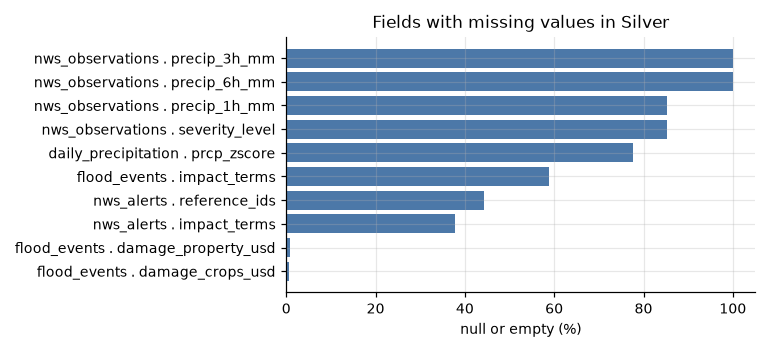
\includegraphics[width=0.8\textwidth]{figures/w3_null_rates.png}
\end{figure}

\begin{figure}[H]
    \centering
    \caption{Outlier analysis: GHCN-Daily wet-day rainfall per station, property damage (log$_{10}$ USD) and event duration (dashed line = IQR fence).}
    \label{fig:outliers}
    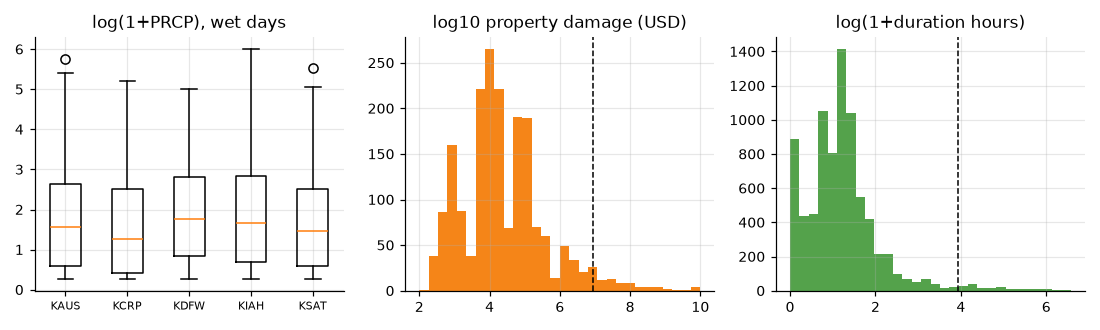
\includegraphics[width=\textwidth]{figures/w3_outliers.png}
\end{figure}

\begin{figure}[H]
    \centering
    \caption{Text length distribution: Storm Events narratives (words, clipped at 150) and NWS alert descriptions.}
    \label{fig:textlen}
    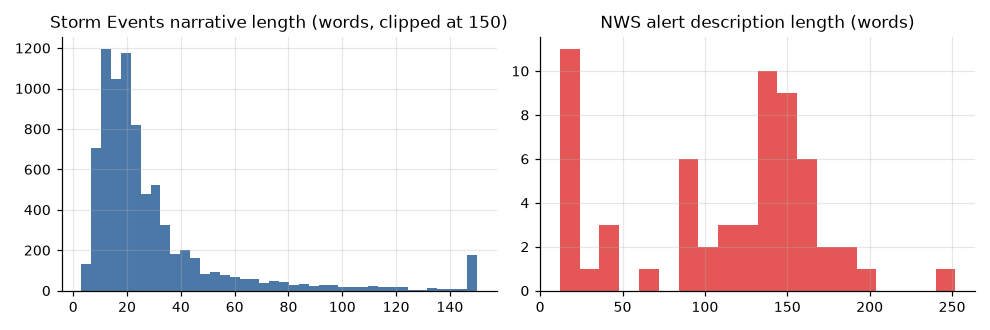
\includegraphics[width=0.9\textwidth]{figures/w3_text_length.png}
\end{figure}

\noindent \textbf{Findings without defects.} The duplicate rate after de-duplication is 0\,\% in every topic, and no record failed a required field, except 3 GHCN-Daily days without a value. These KPIs are kept as \emph{preventive} controls: a future change in a source would show up there first.

% ===========================================================================
\section{\large 4. Governance KPI Definition}
The governance summary is a tidy table with one row per KPI value. Its columns are \texttt{kpi\_group}, \texttt{kpi\_name}, \texttt{topic}, \texttt{field}, \texttt{period\_grain}, \texttt{period\_start}, \texttt{value}, \texttt{numerator}, \texttt{denominator}, \texttt{unit}, \texttt{threshold}, \texttt{status} (ok, warn, fail or info), \texttt{note} and \texttt{gold\_run\_ts}. A dashboard card or chart is a filter on \texttt{kpi\_name}. The KPI groups follow the data-quality dimensions of \citet{wang1996} and ISO/IEC~25012 \citep{iso25012}.

\begin{table}[H]
\centering
\scriptsize
\caption{Governance KPIs: computation in PySpark and justification.}
\label{tab:kpis}
\begin{tabularx}{\textwidth}{>{\raggedright\arraybackslash}p{3.0cm} >{\raggedright\arraybackslash}p{5.6cm} >{\raggedright\arraybackslash}X}
\toprule
\textbf{KPI (group)} & \textbf{Computation (PySpark)} & \textbf{Justification (finding)} \\
\midrule
\texttt{null\_rate} (completeness) & per topic and field: \texttt{sum(isNull)} (or empty array) / rows; threshold 0\,\% for required fields & structural nulls of rainfall and Z-score; damage not estimated \\
\texttt{sentinel\_rate} & share of \texttt{unknown}/\texttt{none}/\texttt{MISSING} in string fields & 85--100\,\% sentinel QC flags; \texttt{flood\_cause} unknown \\
\texttt{station\_day\_completeness} & distinct \texttt{obs\_date} / days between first and last date, per station & 3 missing GHCN-Daily days \\
\texttt{records\_ingested}, \texttt{\_cumulative}, \texttt{records\_by\_event\_period}, \texttt{records\_total}, \texttt{silver\_files} (volume) & \texttt{groupBy} Bronze ingestion day (from the file name), window sum for the cumulative; \texttt{groupBy} event day/year & assignment: volume per source, period and cumulative \\
\texttt{duplicate\_rate\_before\_dedup} (uniqueness) & manifest: (in-batch duplicates + rows already in Silver) / rows offered, per topic and day & 66.5\,\% alerts, 43.2\,\% observations \\
\texttt{duplicate\_rate\_after\_dedup}, \texttt{update\_rate} & rows $-$ distinct (\texttt{event\_id}, \texttt{record\_hash}); share of \texttt{is\_update} & preventive: 0\,\% today \\
\texttt{schema\_compliance\_files} (validity) & each Silver file's Spark schema compared with the expected \texttt{StructType} (names, order, types) & v0.2/v0.3 deviation; key absent vs.\ \texttt{null} \\
\texttt{schema\_compliance\_records}, \texttt{records\_rejected} & manifest: rows written / rows checked; sums by reason (non-flood, required field, outside Texas, out of range, schema) & US5: ``how many records were rejected'' \\
\texttt{outlier\_rate} & flagged rows / rows with a value, per numeric field (IQR, Z-score, NOAA QC, physical range) & GHCN extremes, damage, duration \\
\texttt{text\_length\_words}, \texttt{language\_distribution}, \texttt{encoding\_repaired\_rate} (text) & mean, \texttt{percentile\_approx} median, min, max of word counts per source and year/day; share per language; share of repaired texts & repetition, encoding, alert vs.\ narrative length \\
\texttt{ingestion\_frequency\_compliance}, \texttt{ingestion\_lag\_hours}, \texttt{record\_lag\_hours} (timeliness) & Bronze metadata read with an explicit JSON schema: successful pulls per day vs.\ contract (96, 24, 1); hours since the last successful pull; hours since the newest record & US5: ``when each source was last updated''; GHCN 7-day delay \\
\texttt{precip\_source\_share}, \texttt{maintenance\_flag\_rate} (accuracy) & share per \texttt{precip\_source}; share of \texttt{\$} reports per station & W3-1, W3-2 \\
\bottomrule
\end{tabularx}
\end{table}

\noindent Current values from the Gold run are in Tables~\ref{tab:govtopic}--\ref{tab:goving}.

\begin{table}[H]\centering\scriptsize
\caption{Governance KPIs per Silver topic (\texttt{governance\_20261117\_192000.parquet}). Dup.\ = duplicate rate before / after de-duplication; Schema = schema compliance of files / records; Lag = hours since the newest record.}\label{tab:govtopic}
\begin{tabular}{@{}lrrrrrrr@{}}\toprule
Topic & Records & Files & Dup.\ bef.\ \% & Dup.\ aft.\ \% & Schema f.\ \% & Schema r.\ \% & Lag h\\\midrule
\texttt{nws\_observations} & 372 & 6 & 43.21 & 0 & 100 & 100 & 0.8\\
\texttt{nws\_alerts} & 61 & 2 & 66.48 & 0 & 100 & 100 & 4.9\\
\texttt{daily\_precipitation} & 30,786 & 2 & 0.78 & 0 & 100 & 99.99 & 187.3\\
\texttt{flood\_events} & 8,000 & 1 & 0 & 0 & 100 & 100 & 2,804.0\\
\bottomrule\end{tabular}\end{table}
\begin{table}[H]\centering\scriptsize
\caption{Null-rate and sentinel-rate KPIs above zero (required fields are all 0\,\%).}\label{tab:govnull}
\begin{tabular}{@{}llrp{6.2cm}@{}}\toprule
Topic & Field & \% & Explanation\\\midrule
\texttt{nws\_observations} & \texttt{precip\_3h\_mm} & 100 & only reported in 3/6-hourly METAR\\
\texttt{nws\_observations} & \texttt{precip\_6h\_mm} & 100 & only reported in 6-hourly METAR\\
\texttt{nws\_observations} & \texttt{precip\_1h\_mm} & 85.22 & 5-minute reports never carry rainfall (DQ \#6)\\
\texttt{nws\_observations} & \texttt{severity\_level} & 85.22 & undefined when the rainfall is unknown\\
\texttt{daily\_precipitation} & \texttt{prcp\_zscore} & 77.70 & Z-score only computed on wet days (zero-inflated)\\
\texttt{flood\_events} & \texttt{impact\_terms} & 58.74 & \\
\texttt{nws\_alerts} & \texttt{reference\_ids} & 44.26 & \\
\texttt{nws\_alerts} & \texttt{impact\_terms} & 37.70 & \\
\texttt{flood\_events} & \texttt{damage\_property\_usd} & 0.79 & damage not estimated by NOAA (DQ \#2)\\
\texttt{flood\_events} & \texttt{damage\_crops\_usd} & 0.54 & damage not estimated by NOAA (DQ \#2)\\
\texttt{daily\_precipitation} & \texttt{qflag} (sentinel) & 100 & value replaced by unknown/none/MISSING\\
\texttt{daily\_precipitation} & \texttt{mflag} (sentinel) & 86.58 & value replaced by unknown/none/MISSING\\
\texttt{nws\_observations} & \texttt{qc\_flag} (sentinel) & 85.22 & value replaced by unknown/none/MISSING\\
\texttt{flood\_events} & \texttt{flood\_cause} (sentinel) & 5.62 & value replaced by unknown/none/MISSING\\
\texttt{nws\_observations} & \texttt{text\_description} (sentinel) & 3.49 & value replaced by unknown/none/MISSING\\
\texttt{flood\_events} & \texttt{report\_source} (sentinel) & 0.09 & value replaced by unknown/none/MISSING\\
\bottomrule\end{tabular}\end{table}
\begin{table}[H]\centering\scriptsize
\caption{Other governance KPIs of the Gold run (validity, text, accuracy, timeliness).}\label{tab:govother}
\begin{tabular}{@{}lllrrrl@{}}\toprule
KPI & Topic & Field & Value & Num. & Den. & Status\\\midrule
outlier\_rate & \texttt{nws\_observations} & all\_measurements & 0 & 0 & 372 & info\\
outlier\_rate & \texttt{nws\_observations} & precip\_1h\_mm & -- & -- & 0 & info\\
outlier\_rate & \texttt{nws\_observations} & temperature\_c & 0.27 & 1 & 372 & info\\
outlier\_rate & \texttt{daily\_precipitation} & prcp\_mm (IQR, k=3) & 3.93 & 270 & 6,864 & info\\
outlier\_rate & \texttt{daily\_precipitation} & prcp\_mm (Z-score, |z|>3) & 0.09 & 6 & 6,864 & info\\
outlier\_rate & \texttt{daily\_precipitation} & prcp\_mm (NOAA quality flag) & 0 & 0 & 30,786 & info\\
outlier\_rate & \texttt{flood\_events} & damage\_property\_usd & 3.89 & 74 & 1,900 & info\\
outlier\_rate & \texttt{flood\_events} & duration\_hours & 2.06 & 165 & 8,000 & info\\
language\_distribution & \texttt{flood\_events} & en & 100 & 8,000 & 8,000 & \\
encoding\_repaired\_rate & \texttt{flood\_events} &  & 1.56 & 125 & 8,000 & \\
language\_distribution & \texttt{nws\_alerts} & en & 100 & 61 & 61 & \\
encoding\_repaired\_rate & \texttt{nws\_alerts} &  & 0 & 0 & 61 & \\
ingestion\_lag\_hours & \texttt{nws\_alerts} &  & 0.33 & -- & -- & ok\\
ingestion\_lag\_hours & \texttt{storm\_events\_catalog} &  & 0.33 & -- & -- & ok\\
ingestion\_lag\_hours & \texttt{nws\_observations} &  & 0.33 & -- & -- & ok\\
ingestion\_lag\_hours & \texttt{ghcnd} &  & 8.33 & -- & -- & ok\\
ingestion\_lag\_hours & \texttt{storm\_events\_details} &  & 8.33 & -- & -- & ok\\
station\_day\_completeness & \texttt{daily\_precipitation} & USW00012921 & 99.98 & 6,157 & 6,158 & ok\\
station\_day\_completeness & \texttt{daily\_precipitation} & USW00013904 & 100 & 6,158 & 6,158 & ok\\
station\_day\_completeness & \texttt{daily\_precipitation} & USW00012960 & 100 & 6,157 & 6,157 & ok\\
station\_day\_completeness & \texttt{daily\_precipitation} & USW00003927 & 99.97 & 6,156 & 6,158 & ok\\
station\_day\_completeness & \texttt{daily\_precipitation} & USW00012924 & 100 & 6,158 & 6,158 & ok\\
precip\_source\_share & \texttt{nws\_observations} & missing & 85.22 & 317 & 372 & info\\
precip\_source\_share & \texttt{nws\_observations} & metar\_no\_p\_group & 14.78 & 55 & 372 & info\\
maintenance\_flag\_rate & \texttt{nws\_observations} & KAUS & 8.11 & 6 & 74 & info\\
maintenance\_flag\_rate & \texttt{nws\_observations} & KIAH & 0 & 0 & 77 & info\\
maintenance\_flag\_rate & \texttt{nws\_observations} & KSAT & 12.94 & 11 & 85 & info\\
maintenance\_flag\_rate & \texttt{nws\_observations} & KDFW & 0 & 0 & 69 & info\\
maintenance\_flag\_rate & \texttt{nws\_observations} & KCRP & 5.97 & 4 & 67 & info\\
\bottomrule\end{tabular}\end{table}
\begin{table}[H]\centering\footnotesize
\caption{Ingestion frequency compliance: successful pulls per UTC day against the contract (the stack only ran while the team was working).}\label{tab:goving}
\begin{tabular}{@{}lrrr@{}}\toprule
Source & Expected/day & 2026-11-16 & 2026-11-17\\\midrule
\texttt{bronze\_runs} & 96 & 2 & 7\\
\texttt{ghcnd} & 1 & 1 & 2\\
\texttt{nws\_alerts} & 96 & 2 & 7\\
\texttt{nws\_observations} & 24 & 1 & 5\\
\texttt{storm\_events\_catalog} & 96 & 2 & 7\\
\texttt{storm\_events\_details} & 1 & 1 & 1\\
\bottomrule\end{tabular}\end{table}

\noindent The ingestion compliance is low (2--7\,\% of the 96 expected runs per day) because the Docker stack only ran while the team was working, not 24 hours a day. The KPI makes this visible, which is its purpose; a server deployment would fix it.

% ===========================================================================
\section{\large 5. Storytelling Aggregations and Dashboard Narrative}
\subsection{5.1 Narrative}
We defined the narrative first and then the aggregations that support it. The functional user is the emergency analyst of Workshop~1, and the dashboard tells one story in four steps:
\begin{enumerate}
    \item \textbf{Where} does Texas flood? A few counties concentrate the reports.
    \item \textbf{When?} Floods follow a clear season, with a peak in late spring and a second one in autumn.
    \item \textbf{What} do floods do? Mostly flash floods that close roads and low-water crossings and require water rescues.
    \item \textbf{Is today unusual?} Current rainfall compared with the same station and month in history, active alerts, and the Flood Risk Index per county.
\end{enumerate}
\noindent The key insight the analyst should walk away with is that flood risk in Texas is a matter of recurring places and seasons, triggered by short, intense rain. Today's rainfall only matters when it is unusual for that station and month. The Gold run writes the story as data-driven sentences (section \texttt{narrative}):
\begin{enumerate}
\item Bexar County has the most flood reports since 2010 (322 events, 18.9 per year).
\item May is the peak flood month (115.8 events per year on average).
\item 80\% of the events are flash floods; the most frequent two-word phrase in the narratives is 'heavy rain'.
\item Highest current Flood Risk Index: HIGH in Nueces County (score 3, rainfall of 2026-11-10).
\end{enumerate}

\noindent Our project is about floods, not public opinion. We therefore adapted the suggested ``sentiment'' aggregations: the \emph{severity level} (0--3, defined in Workshop~1) plays the role of the sentiment score of each record, and the narratives of the Storm Events reports play the role of the text corpus.

\subsection{5.2 Aggregations}
The storytelling summary is also a tidy table. Its columns are \texttt{section}, \texttt{metric}, \texttt{user\_story}, \texttt{period\_grain}, \texttt{period\_start}, \texttt{county}, \texttt{station\_id}, \texttt{category}, \texttt{term}, \texttt{value}, \texttt{count}, \texttt{pct}, \texttt{rank}, \texttt{label}, \texttt{latitude}, \texttt{longitude} and \texttt{gold\_run\_ts}. Each section maps to one dashboard element (Table~\ref{tab:sections}).

\begin{table}[H]
\centering
\scriptsize
\caption{Storytelling sections: aggregation, user story and dashboard element.}
\label{tab:sections}
\begin{tabularx}{\textwidth}{>{\raggedright\arraybackslash}p{2.7cm} >{\raggedright\arraybackslash}X >{\raggedright\arraybackslash}p{1.0cm} >{\raggedright\arraybackslash}p{3.0cm}}
\toprule
\textbf{Section} & \textbf{Aggregation (PySpark)} & \textbf{Story} & \textbf{Dashboard element} \\
\midrule
\texttt{headline} & totals: events, events per year, flash-flood share, damage, deaths, counties & US6 & KPI cards \\
\texttt{severity\_distribution} & count and \% per severity level, overall and per year (``sentiment distribution''); alerts per event type & US6, US1 & stacked bars \\
\texttt{trend} & events and average severity per month; damage per month (``sentiment trend'', ``volume trends'') & US6 & time series \\
\texttt{seasonality} & events per year by calendar month & US6 & bar chart \\
\texttt{county\_history} & per county: floods per year, damage, deaths, average severity, rank, centroid; county $\times$ year for the top 15 & US6 & choropleth / map, heat map \\
\texttt{category\_breakdown} & per event type, flood cause and reporting source: count, \%, average severity, damage (``topic breakdown'') & US6 & bars \\
\texttt{source\_comparison} & records and average severity per source (API vs.\ web scraping) & US5 & bars \\
\texttt{keywords} & top 25 unigrams and bigrams (Spark ML pipeline), impact terms: \% of events & US6 & word bars \\
\texttt{keyword\_severity} & share of severe events and average damage per keyword (``keyword sentiment association'') & US6 & bubble chart \\
\texttt{current\_rainfall} & latest 1-, 7-, 30-day rainfall per station (window sums); percentile of the 1-day and 7-day totals against the same station and month in earlier years; NWS METAR 24-hour total & US2, US3 & station cards / gauges \\
\texttt{rain\_climatology} & daily rainfall p50, p90, p95, p99 and \% wet days per station and month & US3 & context band \\
\texttt{alerts} & alerts in effect at the run (superseded messages removed); last 7 days per day, type and county & US1 & alert map, list \\
\texttt{flood\_risk\_index} & index per county with all its inputs & US4 & risk table / map \\
\texttt{fri\_backtest} & hit and false-alarm rates of the index on history, train vs.\ test & US4 & validation panel \\
\texttt{narrative} & four generated sentences & all & story text \\
\bottomrule
\end{tabularx}
\end{table}

\subsection{5.3 Flood Risk Index and its back-test}
The index follows the Workshop~1 rule. The rain level is 3 if $P_{24} \geq 99$ or $R_{24} \geq 75$~mm, 2 if $P_{24} \geq 95$ or $R_{7d} \geq 100$~mm, 1 if $P_{24} \geq 90$, and 0 otherwise. The score is $\max(A, \text{rain level})$ plus 1 when the county is in the top quartile of flood frequency. The FRI is LOW for scores 0--1, MEDIUM for 2 and HIGH for 3 or more. $R_{24}$ is the larger of the latest GHCN-Daily total and the NWS METAR total of the last 24~hours, $P_{24}$ is its percentile against the same station and month in earlier years, and $A$ is the highest alert level in effect in the county.

In the Gold run, Nueces County (Corpus Christi) is HIGH. It received 26.2~mm on 10 November, the 97.7th percentile for November, and 142.6~mm in 7 days (Table~\ref{tab:fri}).
\begin{table}[H]\centering\scriptsize
\caption{Flood Risk Index per county in the Gold storytelling summary (latest GHCN-Daily day).}\label{tab:fri}
\begin{tabular}{@{}llcrrrrrrrrl@{}}\toprule
County & Station & Day & $R_{24}$ & $R_{7d}$ & $P_{24}$ & $A$ & $F$/yr & TopQ & Rain lvl & Score & FRI\\\midrule
Bexar & KSAT & 2026-11-10 & 2 & 37.6 & 88.8 & 0 & 18.9 & 1 & 0 & 1 & \textbf{LOW}\\
Harris & KIAH & 2026-11-09 & 0.3 & 23.4 & 77.5 & 0 & 8.6 & 1 & 0 & 1 & \textbf{LOW}\\
Nueces & KCRP & 2026-11-10 & 26.2 & 142.6 & 97.7 & 0 & 13.5 & 1 & 2 & 3 & \textbf{HIGH}\\
Tarrant & KDFW & 2026-11-10 & 0.5 & 0.5 & 83.8 & 0 & 8.7 & 1 & 0 & 1 & \textbf{LOW}\\
Travis & KAUS & 2026-11-10 & 2.3 & 14.2 & 88.1 & 0 & 9.6 & 1 & 0 & 1 & \textbf{LOW}\\
\bottomrule\end{tabular}\end{table}

\noindent \textbf{Back-test.} Alerts are not available for past years, so only the rainfall and frequency part of the index can be back-tested. We used the 5 station counties from 2010 to 2026, with percentile thresholds from 2010--2020 only, and counted a flood day when Storm Events has a record for that county and local date (Table~\ref{tab:backtest}). The Workshop~1 rule detects 82\,\% of the flood days in the test years, but 90\,\% of its alarms are false. The cause is the frequency term: all five big counties are in the top quartile, so any rain above the 90th percentile already gives MEDIUM. A rainfall-only rule lowers the false alarms a little (86\,\%) but misses more floods (73\,\% hit rate). The index must be recalibrated before Workshop~4, for example by using the 7-day percentile or by requiring an alert for HIGH. The Gold summary already contains the data to compare the options.
\begin{table}[H]\centering\footnotesize
\caption{Back-test of the rainfall + frequency part of the index (5 counties, county-days 2010--2026; thresholds from 2010--2020). W1 rule: alarm when rain level + top-quartile term $\geq$ 2; rain-only rule: alarm when rain level $\geq$ 2.}\label{tab:backtest}
\begin{tabular}{@{}llrrrr@{}}\toprule
Rule & Period & Flood days & Hit rate \% & Alarm days & False alarms \%\\\midrule
W1 rule & test 2021- & 138 & 81.88 & 1,192 & 90.52\\
W1 rule & train 2010-2020 & 306 & 84.31 & 2,353 & 89.04\\
rain-only rule & test 2021- & 138 & 73.19 & 729 & 86.15\\
rain-only rule & train 2010-2020 & 306 & 71.90 & 1,409 & 84.39\\
\bottomrule\end{tabular}\end{table}

% ===========================================================================
\section{\large 6. PySpark Implementation}
\subsection{6.1 Spark session and Docker adjustments}
PySpark runs in \textbf{local mode} inside the Airflow scheduler container. With the \texttt{LocalExecutor}, the scheduler runs the tasks, so no cluster and no extra container are needed. Table~\ref{tab:sparkconf} shows the session configuration of \texttt{flood\_monitor/gold/spark.py}.

\begin{table}[H]
\centering
\scriptsize
\caption{Spark session configuration (\texttt{get\_spark()}).}
\label{tab:sparkconf}
\begin{tabularx}{\textwidth}{>{\raggedright\arraybackslash}p{4.4cm} >{\raggedright\arraybackslash}p{3.0cm} >{\raggedright\arraybackslash}X}
\toprule
\textbf{Setting} & \textbf{Value} & \textbf{Reason} \\
\midrule
\texttt{master} & \texttt{local[*]} & one thread per CPU core of the container \\
\texttt{spark.driver.memory} & 1g (\texttt{SPARK\_DRIVER\_MEMORY}) & in local mode the driver is the only JVM; the inputs are about 8~MB of Parquet \\
\texttt{spark.sql.shuffle.partitions} & 8 & the default 200 would create hundreds of tiny tasks \\
\texttt{spark.sql.session.timeZone} + JVM \texttt{-Duser.timezone} & UTC & dates match the Silver UTC timestamps \\
\texttt{spark.ui.enabled} & false & no web UI port inside Airflow \\
\texttt{spark.local.dir} & \texttt{/tmp/\allowbreak spark-local} & shuffle files outside the mounted data lake \\
\texttt{PYSPARK\_PYTHON} & interpreter of the task & workers and driver must use the same Python \\
\bottomrule
\end{tabularx}
\end{table}

\noindent \textbf{Docker changes.}
\begin{itemize}
    \item The \texttt{Dockerfile} installs \texttt{openjdk-17-jre-headless} as root, because Spark~3.5 needs Java 8, 11 or 17. It also links \texttt{JAVA\_HOME} to a fixed path, so the image works on Intel and Apple-Silicon laptops.
    \item \texttt{requirements-airflow.txt} adds \texttt{pyspark}, pinned to 3.5.2 by the Airflow constraints file.
    \item \texttt{docker-compose.yml} adds the \texttt{SPARK\_*} variables and \texttt{GOLD\_KEEP\_RUNS}.
    \item \texttt{datalake\_gold/} was already mounted as a volume in Workshop~2.
\end{itemize}
To apply the changes, run \texttt{docker compose up -d --build}.

\subsection{6.2 Gold DAG}
\texttt{airflow/dags/gold\_processing\_dag.py} (TaskFlow API) runs every hour at minute 20 (\texttt{20 * * * *}), after the Bronze run (minutes 00 and 15) and the Silver run (every 10 minutes). The storytelling summary changes slowly, but the alerts (US1) and the index (US4) must be recent. A run takes about 2 minutes on the test machine.
\begin{enumerate}
    \item \texttt{check\_silver\_inputs} lists the Silver files per topic, and fails if a topic has none.
    \item \texttt{build\_governance\_summary} and then \texttt{build\_storytelling\_summary} each run one Spark session and stop it. They run one after the other, so that only one JVM is alive at a time on a laptop.
    \item \texttt{validate\_gold\_outputs} reads both files back with PyArrow, as the dashboard will, and checks that every KPI group and story section is present.
    \item \texttt{record\_gold\_manifest} writes the lineage (the Silver files read and the files produced) to \texttt{\_gold\_manifest.jsonl}, and keeps the newest 48 runs of each summary.
\end{enumerate}
Retries: 1 after 3 minutes; timeout: 30 minutes. File names: \texttt{governance\_YYYYMMDD\_HHMMSS.parquet} and \texttt{storytelling\_YYYYMMDD\_HHMMSS.parquet}, where the timestamp is the UTC end of the data interval, as in Bronze.

\subsection{6.3 Key transformations}
\begin{itemize}
    \item \textbf{Folder read.} \texttt{spark.read.option("pathGlobFilter", "<topic>\_*.parquet").option("mergeSchema", "true").parquet("datalake\_silver/")} reads every file of a topic as one DataFrame. Spark ignores files starting with ``\_'', so the manifest and the key registry do not interfere.
    \item \textbf{Latest version.} A window \texttt{row\_number()} partitioned by \texttt{event\_id} and ordered by \texttt{processed\_at\_utc} keeps the newest version of each record (Silver keeps changed records as \texttt{is\_update}).
    \item \textbf{Rainfall windows and percentiles.} Range windows of 7 and 30 days over the day number give $R_{7d}$ and $R_{30d}$. A self-join on station and month against earlier years gives the percentile ranks, and \texttt{percentile\_approx} gives the monthly climatology.
    \item \textbf{NLP in Spark ML.} A \texttt{Pipeline} with \texttt{RegexTokenizer}, \texttt{StopWordsRemover} (our 117 domain stop words plus English) and \texttt{NGram(n=2)}. Bigrams are built before stop-word removal and kept only when both words are content words, so ``rain \ldots{} flash'' is never a bigram \citep{manning2008}. Higher-order SQL functions (\texttt{filter}) drop tokens with digits.
    \item \textbf{Governance from metadata.} The Silver manifest is parsed by Spark's JSON reader. The Bronze metadata is read with an explicit nested schema, so Spark does not parse the 17~MB payloads into columns.
    \item \textbf{Single-file output.} Each block is materialized with \texttt{localCheckpoint()} and joined with \texttt{unionByName}, then \texttt{coalesce(1)} writes one part file, which is renamed to the timestamped name (Spark always writes a folder).
\end{itemize}

% ===========================================================================
\section{\large 7. Results Evidence}
The Gold DAG ran successfully on 17 November 2026 (run 19:20 UTC), after a Bronze run at 19:00 and a Silver run at 19:10 that processed it. The validation task logged \texttt{governance\_rows=\GovRows}, \texttt{storytelling\_rows=\StoryRows}, \texttt{kpi\_fail=[]} and \texttt{errors=[]}. Figures~\ref{fig:govcontent} and~\ref{fig:storycontent} show the content of the two Gold Parquet files read with Pandas, and Figure~\ref{fig:preview} is the preview of \texttt{notebooks/04\_gold\_preview.ipynb}.

\begin{figure}[H]
    \centering
    \caption{Content of the Gold governance file (sample of rows read with Pandas).}
    \label{fig:govcontent}
    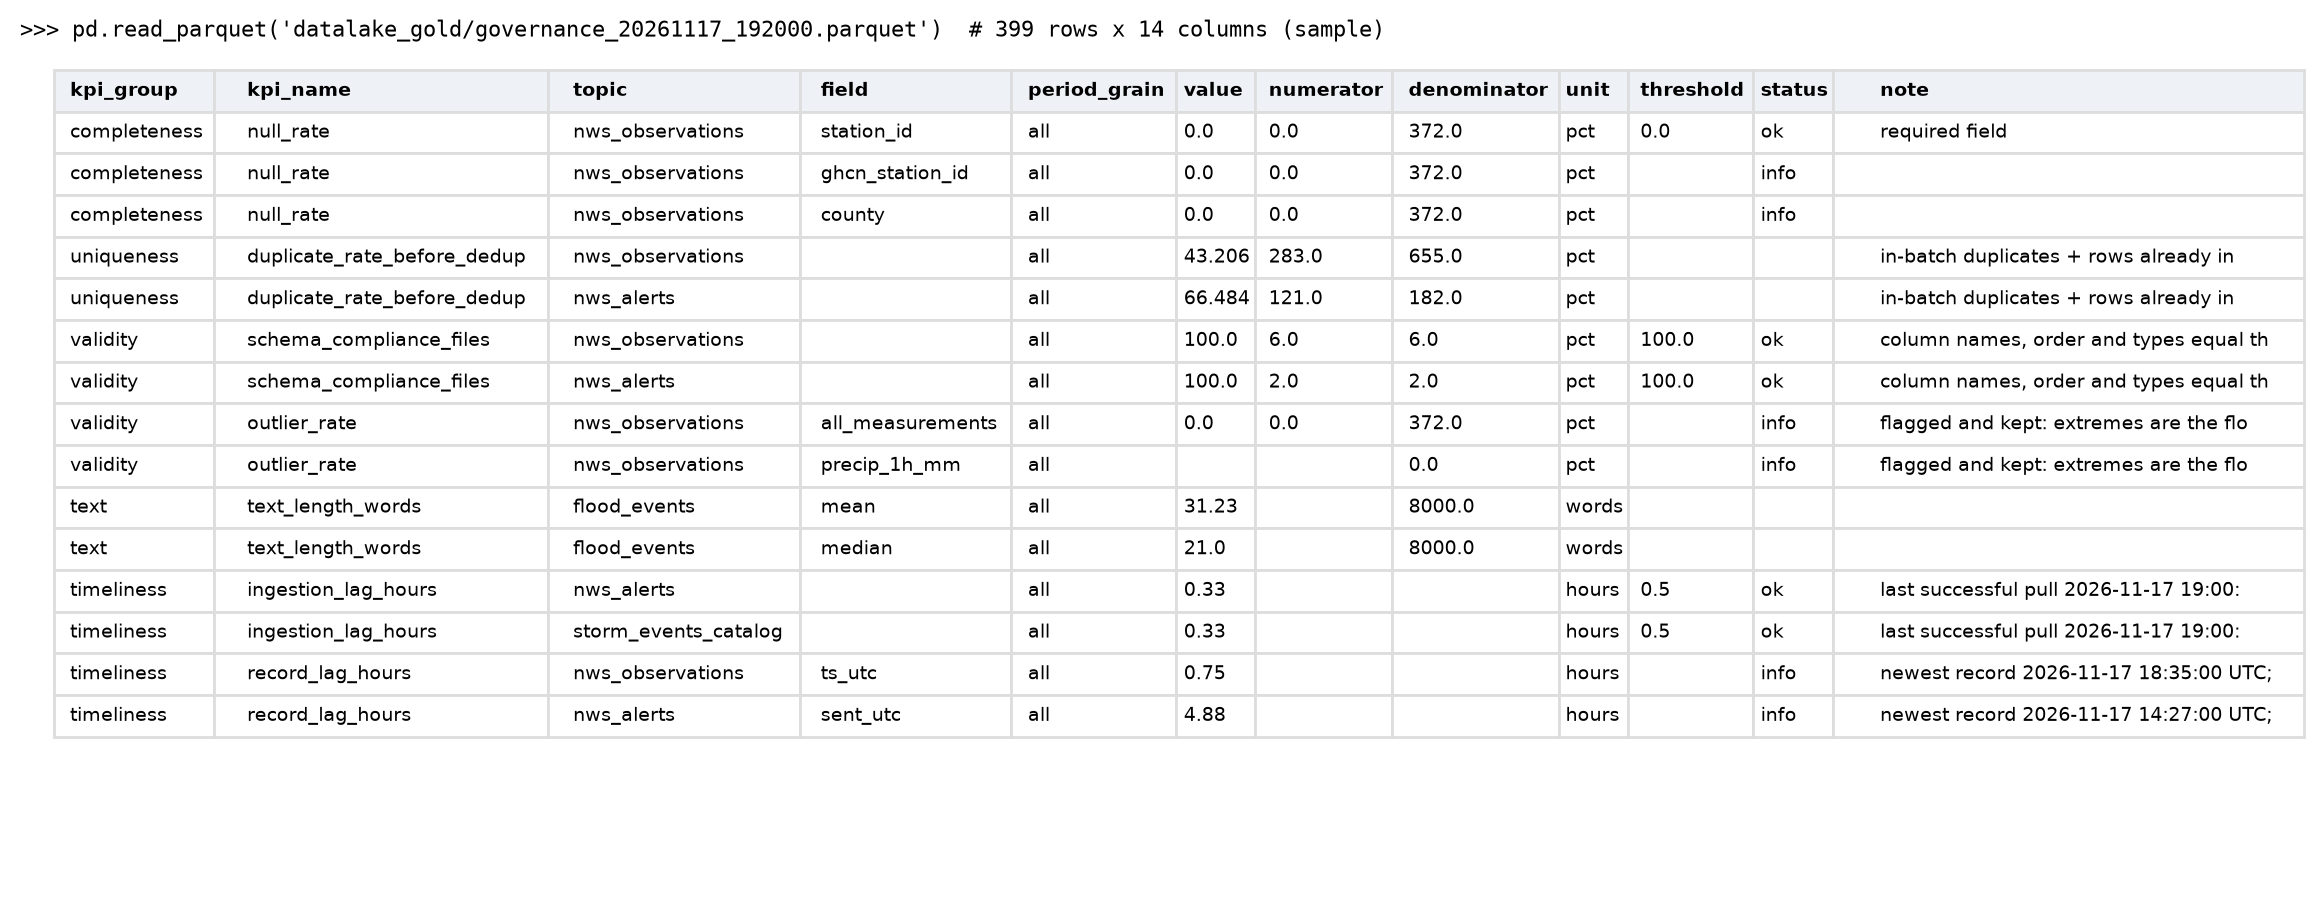
\includegraphics[width=\textwidth]{figures/gold_governance_content.png}
\end{figure}

\begin{figure}[H]
    \centering
    \caption{Content of the Gold storytelling file (sample of rows read with Pandas).}
    \label{fig:storycontent}
    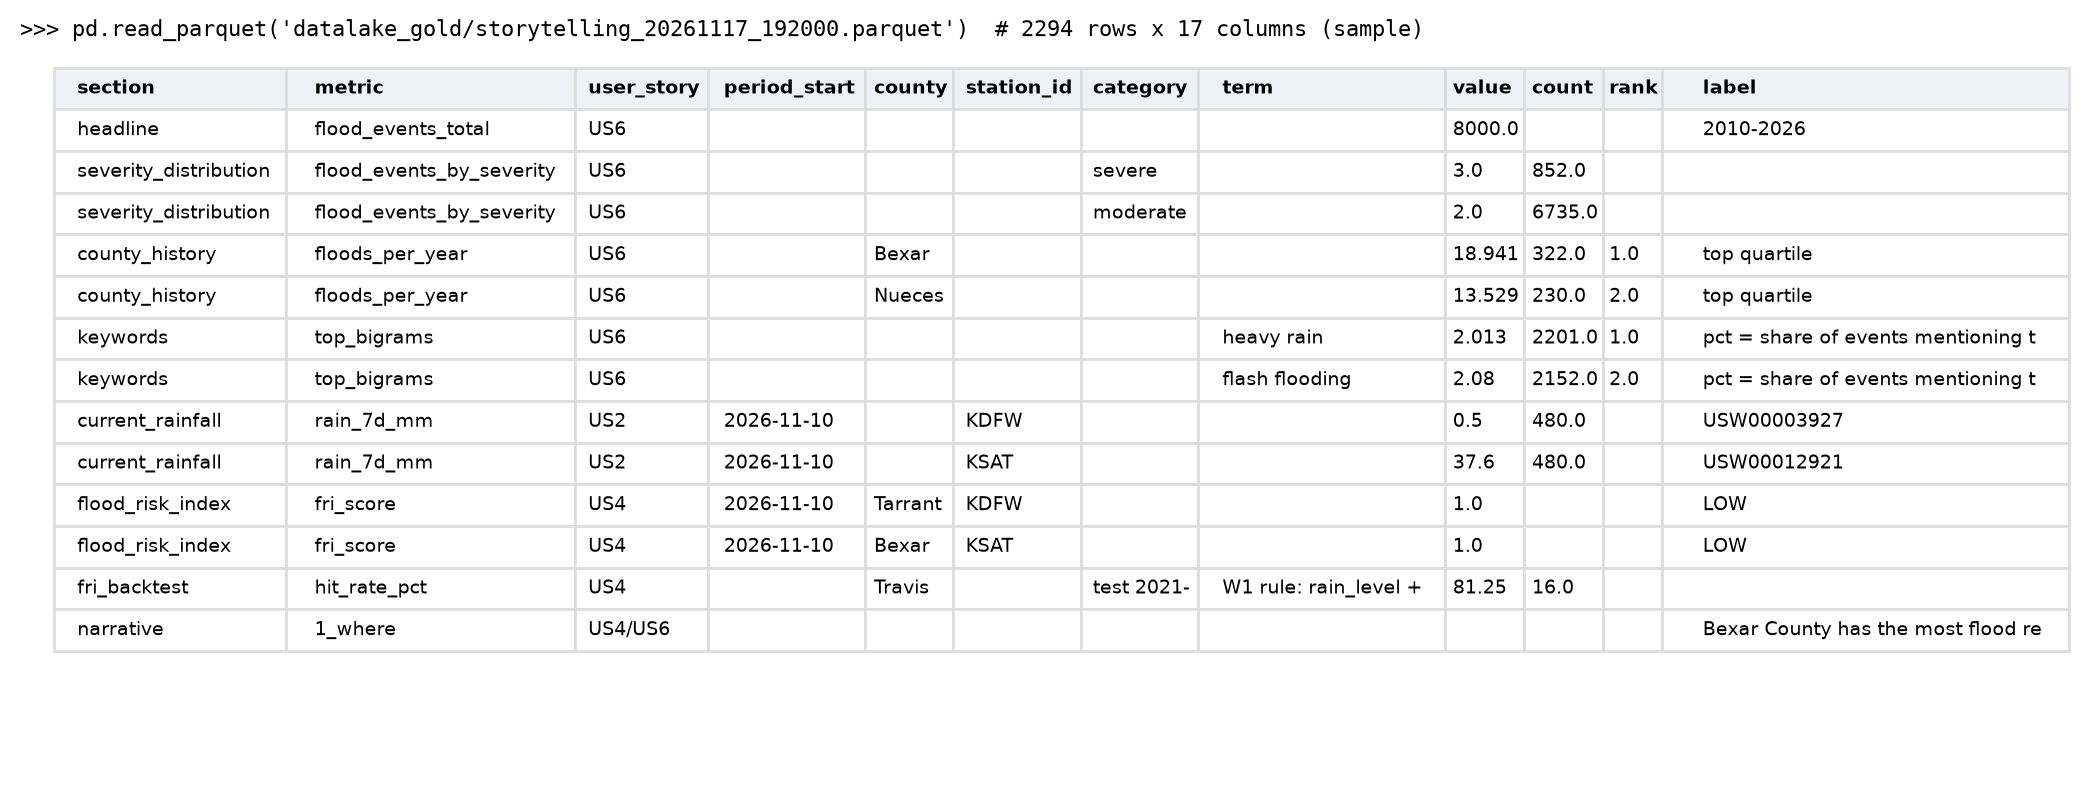
\includegraphics[width=\textwidth]{figures/gold_storytelling_content.png}
\end{figure}

\begin{figure}[H]
    \centering
    \caption{Storytelling summary preview (notebook 04): severity distribution, seasonality, top counties and top bigrams.}
    \label{fig:preview}
    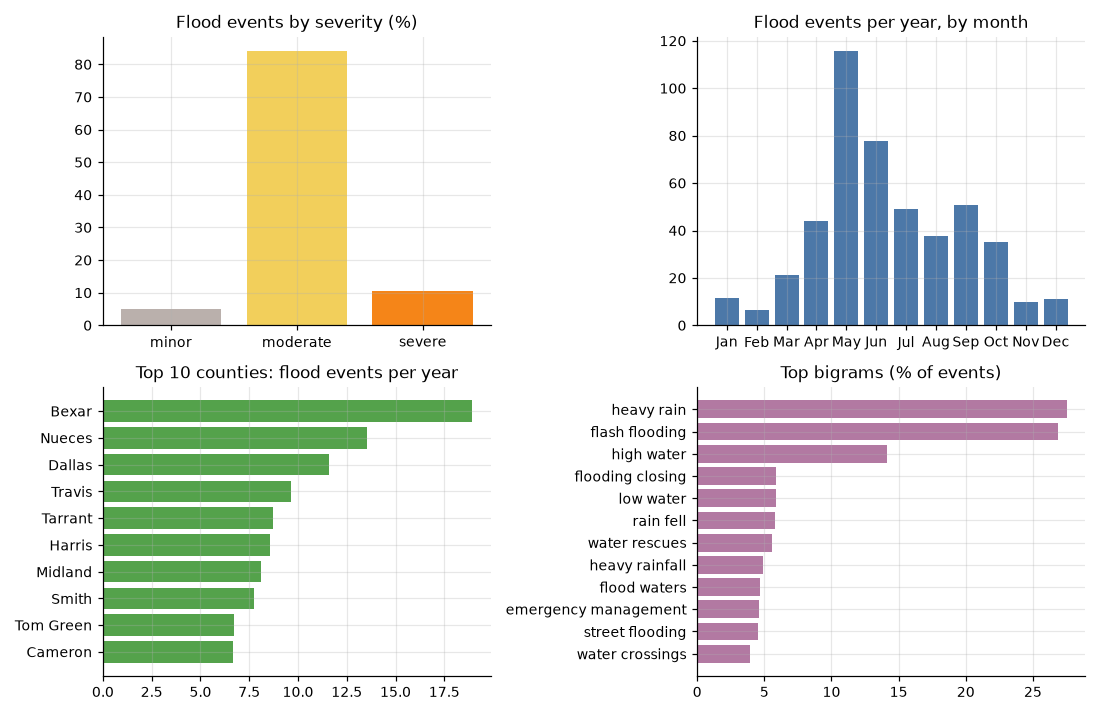
\includegraphics[width=0.9\textwidth]{figures/w3_gold_storytelling_preview.png}
\end{figure}

\shot{airflow_dags_list_w3.png}{Airflow Web UI with the three DAGs (Bronze, Silver and Gold) and their successful runs.}
\shot{gold_dag_graph.png}{Graph view of a successful gold\_flood\_processing\_dag run.}
\shot{gold_dag_grid.png}{Grid view of gold\_flood\_processing\_dag runs.}
\shot{gold_spark_log.png}{Log of build\_governance\_summary showing the Spark session (local mode) and the Gold file written.}

\noindent\textbf{Gold manifest} (lineage of the run, trimmed):
\lstinputlisting{generated/gold_manifest.txt}

% ===========================================================================
\section{\large 8. Experimentation Log: What Did Not Work}
\begin{itemize}
    \item \textbf{Reading the whole Silver folder.} A plain \texttt{spark.read.parquet("datalake\_silver/")} returned 39,219 rows with only 20 columns: Spark took the schema of one file (GHCN-Daily) and silently lost the columns of the other topics. With \texttt{mergeSchema} it returned 96 mixed columns. Hence the per-topic file filter, and the Silver replay to v0.3 so that all files of a topic share one schema.
    \item \textbf{Reading the manifest with Spark.} \texttt{spark.read.json("\_manifest.jsonl")} failed with \texttt{UNABLE\_TO\_INFER\_SCHEMA}, because Hadoop treats names starting with ``\_'' as hidden. The lines are now passed to Spark's JSON reader as an RDD of strings.
    \item \textbf{Python version mismatch.} The first local test failed with \texttt{PYTHON\_VERSION\_MISMATCH} (driver 3.12, worker 3.13). \texttt{PYSPARK\_PYTHON} is now set to the interpreter of the Airflow task.
    \item \textbf{Slow storytelling job.} The first version built about 60 aggregations and joined them with \texttt{unionByName}. Every action re-planned and re-computed the whole lineage (task binaries of 1.9~MB), and the job took 243~s. With one \texttt{localCheckpoint()} per block it takes 51--57~s.
    \item \textbf{Cached DataFrames.} \texttt{input\_file\_name()} and \texttt{inputFiles()} return nothing on a cached DataFrame, so the first \texttt{silver\_files} KPI was 0 or 1. The file count is now taken before caching.
    \item \textbf{Bigrams across stop words.} After stop-word removal, ``heavy rain that led to flash flooding'' produced the false bigram ``rain flash'' (1,197 events). Bigrams are now built before stop-word removal.
    \item \textbf{Active alerts.} The first version listed six versions of the same McMullen County Flood Warning, because the references never matched the alert identifiers (W3-7).
    \item \textbf{Flood Risk Index.} The back-test showed 90\,\% false alarms (Section~5.3). The rule is kept as defined in Workshop~1 and flagged for calibration.
\end{itemize}

\section{\large 9. Conclusions and Next Steps}
The Medallion pipeline now has three working layers. Bronze is incremental and checks for schema drift; Silver v0.3 fixes ten observed problems and records its own quality counters; and Gold (PySpark) produces a governance summary and a storytelling summary that will be the only data source of the Plotly Dash dashboards in Workshop~4. Every KPI comes from an observed problem, and every story section comes from a user story. Next steps: run the stack continuously to reach the ingestion contract, recalibrate the Flood Risk Index with the back-test data, and map each Gold section to its chart in the two Dash applications.

\newpage
% Referencias
\renewcommand\refname{\large\textbf{References}}
\nocite{*}
\bibliography{mibibliografia}

\end{document}
